\documentclass[14pt]{extarticle}

\begin{document}
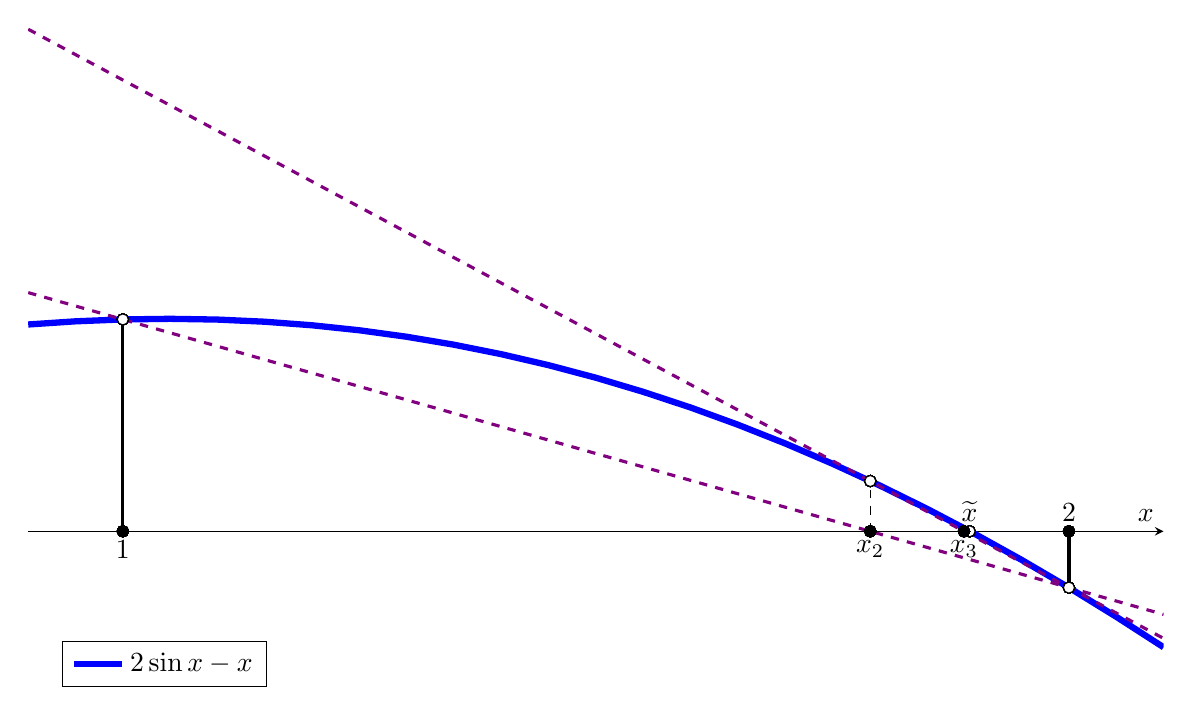
\begin{tikzpicture} [
	declare function= {
		u(\x) = 2*sin(\x / pi * 180) -\x;
		dydx(\a,\b) = (u(\b)-u(\a)) / (\b-\a);
		chorde(\x,\a,\b) = dydx(\a,\b) * (\x-\b) + u(\b);
		xn(\a,\b) = \b - u(\b)/dydx(\a,\b);
	},]
	\begin{axis} [
		height=11cm,
		width=16cm,
		xlabel = {$x$},
		ylabel = {$y$},
		axis x line = middle,
		hide y axis,
		domain = 0.9:2.1,
		ticks = none,
		legend pos = south west ]

		\newcommand*{\varA}{1}
		\newcommand*{\varB}{2}
		\newcommand*{\trueX}{1.895}
		\pgfmathsetmacro{\fa}{u(\varA)}
		\pgfmathsetmacro{\fb}{u(\varB)}
		\pgfmathsetmacro{\Xzeroth}{\varA}
		\pgfmathsetmacro{\Xfirst}{\varB}
		\pgfmathsetmacro{\Xsecond}{xn(\Xzeroth,\Xfirst)}
		\pgfmathsetmacro{\Xthird}{xn(\Xfirst,\Xsecond)}
		\pgfmathsetmacro{\fXzeroth}{u(\Xzeroth)}
		\pgfmathsetmacro{\fXfirst}{u(\Xfirst)}
		\pgfmathsetmacro{\fXsecond}{u(\Xsecond)}
		\pgfmathsetmacro{\fXthird}{u(\Xthird)}

		\addplot[color=blue, line width=.08cm]{u(x)};
		\addplot[color=violet, line width=.04cm, dashed]
			{chorde(x,\Xzeroth,\Xfirst)};
		\addplot[color=violet, line width=.04cm, dashed]
			{chorde(x,\Xfirst,\Xsecond)};

		\coordinate(A) at 	(\varA,		\fa);
		\node[below](Ap) at	(\varA,		0) {$\varA$};
		\coordinate(B) at 	(\varB,		\fb);
		\node[above](Bp) at	(\varB,		0) {$\varB$};
		\node[above](X) at	(\trueX,	0)
			{$\widetilde{x}$};
		\coordinate(X0) at 	(\Xzeroth,	\fXzeroth);
		\coordinate(X0p) at	(\Xzeroth,	0);
		\coordinate(X1) at 	(\Xfirst,	\fXfirst);
		\coordinate(X1p) at	(\Xfirst,	0);
		\coordinate(X2) at 	(\Xsecond,	\fXsecond);
		\node[below](X2p) at	(\Xsecond,	0) {$x_2$};
		\coordinate(X3) at 	(\Xthird,	\fXthird);
		\node[below](X3p) at	(\Xthird,	0) {$x_3$};

		\addplot[mark=*,only marks, fill=white]
			(\trueX,0) node[above, pos=1]{};
		\addplot[mark=*,only marks, fill=white]
			(\Xzeroth,\fXzeroth) node[above, pos=1]{};
		\addplot[mark=*,only marks, fill=white]
			(\Xfirst,\fXfirst) node[above, pos=1]{};
		\addplot[mark=*,only marks, fill=white]
			(\Xsecond,\fXsecond) node[above, pos=1]{};
		\addplot[mark=*,only marks, fill=black]
			(\varA,0) node[above, pos=1]{};
		\addplot[mark=*,only marks, fill=black]
			(\varB,0) node[above, pos=1]{};
		\addplot[mark=*,only marks, fill=black]
			(\Xsecond,0) node[above, pos=1]{};
		\addplot[mark=*,only marks, fill=black]
			(\Xthird,0) node[above, pos=1]{};

		\draw[very thick] (Ap) -- (A)	(Bp) -- (B);
		%\draw[-latex, dashed, red, thick] (X0) -- (X1p);
		\draw[dashed] (X2p) -- (X2);

		\addlegendentry{$2\sin x-x$};
	\end{axis}
\end{tikzpicture}
\end{document}
